\documentclass{sig-alternate-05-2015}


\usepackage[utf8]{inputenc}
\usepackage[T1]{fontenc}
\usepackage{hyperref}
\usepackage{booktabs}

\usepackage{subcaption}
\usepackage{cleveref}
\usepackage{ucs}
\usepackage{framed}

\usepackage[labelfont=bf]{caption}

\hypersetup{
    colorlinks,
    linkcolor={red!65!black},
    citecolor={blue!50!black},
    urlcolor={blue!80!black}
}

\usepackage{listings}  

% ARIAL
%\usepackage{helvet}
%\renewcommand{\familydefault}{\sfdefault}


% TIMES
\usepackage{mathptmx}% http://ctan.org/pkg/mathptmx

\usepackage{pgfplots, pgfplotstable}

\usepackage{xcolor}

\definecolor{orange}{RGB}{230, 100, 20}
\definecolor{gruen}{RGB}{255, 190, 69}

\definecolor{RYB1}{HTML}{8F83DB}
\definecolor{RYB2}{HTML}{DDDDDD}
\definecolor{RYB3}{HTML}{FFFFFF}

\definecolor{RYB4}{HTML}{A699FF}
\definecolor{RYB5}{HTML}{FFBA49}
\definecolor{RYB6}{HTML}{FFFFFF}


\definecolor{RYB7}{HTML}{6A62A3}
\definecolor{RYB8}{HTML}{BEB4FF}
\definecolor{RYB9}{HTML}{E6E3FF}

\definecolor{RYB10}{HTML}{FFB030}
\definecolor{RYB11}{HTML}{FFCD7C}

\pgfplotscreateplotcyclelist{ColorListBar}{
{fill=RYB1},
{fill=RYB2},
{fill=RYB3},
}


\pgfplotscreateplotcyclelist{ColorListBar2}{
{fill=RYB4},
{fill=RYB5},
{fill=RYB6},
}

\pgfplotscreateplotcyclelist{ColorListBar3}{
{fill=RYB7},
{fill=RYB8},
{fill=RYB9},
}


\begin{document}
\lstset{
	language=PHP,
	basicstyle=\footnotesize\ttfamily,
    commentstyle = \color{gray},
    extendedchars = \true,
    inputencoding = utf8x,
    keepspaces = true,
    keywordstyle = \bfseries
}

% Copyright
\setcopyright{acmcopyright}
%\setcopyright{acmlicensed}
%\setcopyright{rightsretained}
%\setcopyright{usgov}
%\setcopyright{usgovmixed}
%\setcopyright{cagov}
%\setcopyright{cagovmixed}


% DOI
\doi{10.475/123_4}

% ISBN
\isbn{123-4567-24-567/08/06}

%Conference
\conferenceinfo{ISSTA '17}{July 9--13, 2013, Santa Barbara, CA, USA}

\acmPrice{\$15.00}

%
% --- Author Metadata here ---
\conferenceinfo{ISSTA '17}{July 9--13, 2013, Santa Barbara, CA, USA}
%\CopyrightYear{2007} % Allows default copyright year (20XX) to be over-ridden - IF NEED BE.
%\crdata{0-12345-67-8/90/01}  % Allows default copyright data
% (0-89791-88-6/97/05) to be over-ridden - IF NEED BE.
% --- End of Author Metadata ---

\title{Does It Scale? Static Output Approximation of PHP Web Applications Using
Symbolic Execution} 

%


\numberofauthors{3} %  in this sample file, there are a *total*
% of EIGHT authors. SIX appear on the 'first-page' (for formatting
% reasons) and the remaining two appear in the \additionalauthors section.
%
\author{
% You can go ahead and credit any number of authors here,
% e.g. one 'row of three' or two rows (consisting of one row of three
% and a second row of one, two or three).
%
% The command \alignauthor (no curly braces needed) should
% precede each author name, affiliation/snail-mail address and
% e-mail address. Additionally, tag each line of
% affiliation/address with \affaddr, and tag the
% e-mail address with \email.
%
% 1st. author
\alignauthor
Stefan Mühlbauer\\
       \affaddr{TU Braunschweig, Germany}\\
       %\email{s.muehlbauer@tu-bs.de}
% 2nd. author
\alignauthor
%Christian Kästner\\
%      \affaddr{Carnegie Mellon University, USA}\\
       %\email{ckaestner@cs.cmu.edu}
% 3rd. author
\alignauthor
%Tien N. Nguyen\\
%       \affaddr{University of Texas at Dallas, USA}\\
%      %\email{tien.n.nguyen@utdallas.edu}
}
% There's nothing stopping you putting the seventh, eighth, etc.
% author on the opening page (as the 'third row') but we ask,
% for aesthetic reasons that you place these 'additional authors'
% in the \additional authors block, viz.
\additionalauthors{Additional authors: John Smith (The Th{\o}rv{\"a}ld Group,
email: {\texttt{jsmith@affiliation.org}}) and Julius P.~Kumquat
(The Kumquat Consortium, email: {\texttt{jpkumquat@consortium.net}}).}
\date{30 July 1999}
% Just remember to make sure that the TOTAL number of authors
% is the number that will appear on the first page PLUS the
% number that will appear in the \additionalauthors section.

\maketitle
\begin{abstract}
Dynamic web applications have become widely popular and are to a large
proportion based on the scripting language PHP. Output approximation of web
applications enables a range of additional tool support as well as possibilities
for vulnerability detection. Unfortunately, recent approximation approaches have
only been evaluated for smaller systems due to both conceptual limitations and
unsupported language features.

This paper presents an experience report about the scalability of output
approximation using symbolic execution of state-of-the-art PHP web
applications. For a symbolic execution engine extended with support for
object-oriented programming and arrays, we identified language features and
corresponding programming patterns that impede symbolic execution and limit the
scalability of this approach. Our findings include: (1) dynamic features such as
functions and includes are prone to fail for certain programming patterns. (2)
Expressions containing elements from I/O, databases or files can heavily impede
symbolic execution. Our findings provide useful guidelines to design new
tools and also to improve the development process of statically analyzable web
applications.

\end{abstract}


%
% The code below should be generated by the tool at
% http://dl.acm.org/ccs.cfm
% Please copy and paste the code instead of the example below. 
%
\begin{CCSXML}
<ccs2012>
 <concept>
  <concept_id>10010520.10010553.10010562</concept_id>
  <concept_desc>Computer systems organization~Embedded systems</concept_desc>
  <concept_significance>500</concept_significance>
 </concept>
 <concept>
  <concept_id>10010520.10010575.10010755</concept_id>
  <concept_desc>Computer systems organization~Redundancy</concept_desc>
  <concept_significance>300</concept_significance>
 </concept>
 <concept>
  <concept_id>10010520.10010553.10010554</concept_id>
  <concept_desc>Computer systems organization~Robotics</concept_desc>
  <concept_significance>100</concept_significance>
 </concept>
 <concept>
  <concept_id>10003033.10003083.10003095</concept_id>
  <concept_desc>Networks~Network reliability</concept_desc>
  <concept_significance>100</concept_significance>
 </concept>
</ccs2012>  
\end{CCSXML}

\ccsdesc[500]{Computer systems organization~Embedded systems}
\ccsdesc[300]{Computer systems organization~Redundancy}
\ccsdesc{Computer systems organization~Robotics}
\ccsdesc[100]{Networks~Network reliability}



%
%  Use this command to print the description
%
\printccsdesc

% We no longer use \terms command
%\terms{Theory}

\keywords{Static program behavior, Static metrics, Dynamic language features,
Static Analysis, PHP}

\section{Introduction}
Dynamic web applications have become widely popular and various different
implementation techniques have emerged, ranging from server-side scripting
languages to state-of-the-art frameworks for web development. For scritpting
languages such as PHP, source code usually contains script code along with nested
target code since the HTML pages are dynamically generated.


\section{State Of the Art}
\subsection{Symbolic Execution (and Choices?)}
\subsection{Use Cases for Output Approximation}

\begin{figure}
	
	\centering
	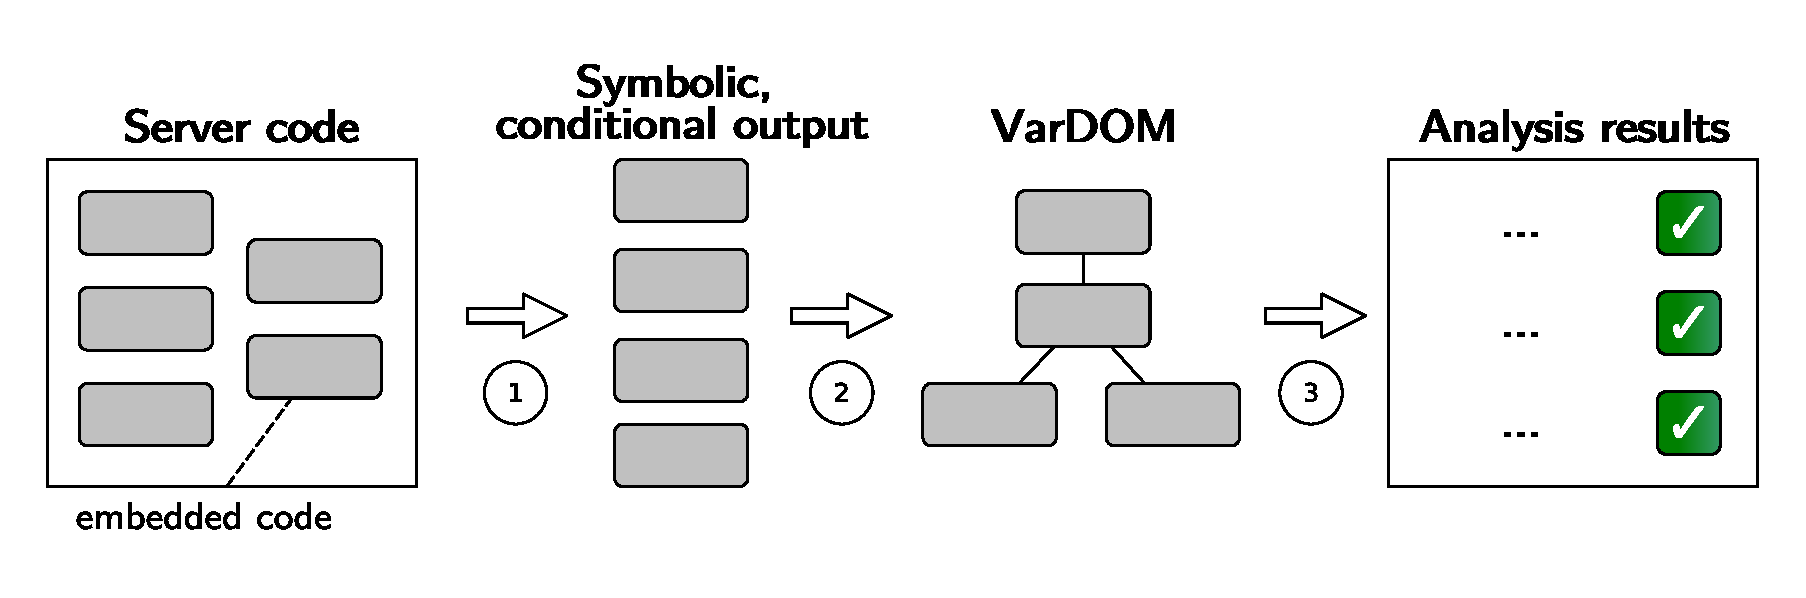
\includegraphics[width=0.5\textwidth]{images-paper/approach}
	\caption{Approach overview; the different analyses in Varis are based upon the
	symbolic output. Step 1 is the \emph{symbolic execution}, step 2 is the
	\emph{variability-aware parsing} and step enfolds subsequent analyses based
	upon the symbolic output.}
	\label{approach}
\end{figure}

\begin{itemize}
  \item Steps: Symbolic Execution $\rightarrow$ Parsing $\rightarrow$
  Analysis, see Figure \ref{approach}
  \item Varis: IDE support \cite{Nguyen:2015:VIS:2819009.2819140} for PHP with
  code slicing \cite{Nguyen:2015:CPS:2786805.2786872}, code navigation
  \cite{Nguyen:2014:BCG:2635868.2635928} and
  HTML validation \cite{Nguyen:2011:AFH:2190078.2190142}.
\end{itemize}

\section{Towards scalable symbolic execution}
\subsection{Can we have a practical tool?}
\begin{itemize}
  \item Are the assumprions just engineering or do not matter for accuracy? 
\end{itemize}
\subsection{Oak: A Symbolic Interpreter}
\begin{itemize}
  \item \textsc{Oak}\footnote{\url{https://github.com/smba/oak}}:
  Re-implementing and extending the symbolic execution engine with OOP and array support
  \item Test-driven implementation strategy 
  \item WordPress!
\end{itemize}
\subsection{Experience Report}
\subsubsection{Problems}
\subsubsection{Concrete/Symbolic Boundary}
\subsubsection{Further experiments}
\begin{itemize}
  \item SPL approach for Oak in order to evaluate different execution modes
  (feature model?)
  \item ``\emph{Things we tried, some improvement but had no significant impact;
  tradeoffs between accuracy and performance etc.}''
\end{itemize}

\section{How can we explain low code coverage?}
As already stated in the previous section, we encountered sevaral problems
during the development of the symbolic interpreter. Therefore this section
describes our methods to evaluate the precision of the output approximation, and
possible explanation theses.

\subsection{How to measure approximation success?} \label{heuristic}
In the absence of ground truth for the approximated output we
are bound to choose a \emph{heuristic approach} in order to measure the accuracy
of the aproximation. We define a string literal to be an \emph{output candidate} if there exists an
execution path reaching the string literal and passing it to an 
output-generating statement (e.g., \texttt{echo} or \texttt{print}).

We approximate output candidates as those string literals containing the
characters \texttt{<}, \texttt{>} or both. We evaluated this heuristic manually
with a sample of 400 string literals from the entire corpus and measured a
precision of 94\% and a recall of 50\%. This means, our classification has a
rate of 6\% false positives and only half of the actual output candidates
respond. These were mostly HTML-containing literals, whereas plain text did not
respond. 

\subsection{Experimental Evaluation} 
For the evaluation we chose to selected a corpus of twelve PHP systems with regard to
previous work, but chose to additionally scale system size and recency. The full list of twelve PHP systems is shown in Table \ref{corpus}. Our selection contains
twelve systems:

\begin{itemize}
  \item Four small-scale/old systems are systems that have been subject to
  related studies and approaches in order to have comparable results. These
  projects do not make comprehensive use of PHP language features and output
  approximation on these systems achieved fairly high precision
  \cite{minamide2005static,Nguyen:2014:BCG:2635868.2635928}.
  
  \item Three large-scale/modern systems that have been subject to related
  studies, especially their use of language features as we aim to study
  scalability of symbolic execution The feature usage of these systems has been
  studied by Hills et al. \cite{Hills:2013:ESP:2483760.2483786}
  
  \item Five small-scale/modern systems to compare the impact
  of system size to the second part of the corpus. The systems are selected
  from a list of recent content management systems (CMS) \cite{codegeekz}. We only selected five systems 	due to limited support of the Quercus parser used in our implementation.
\end{itemize}

\begin{table*}[t]
\centering 
	\begin{tabular}{p{4cm}rrrl}
	\toprule
	\textbf{System} & \textbf{Version} & \textbf{File Count} & \textbf{SLOC} &
	\textbf{Description}
	\\
	\midrule
	AddressBook & 8.2.5.2 & 239 & 51,907 & Adress Administration \\
	SchoolMate & 1.5.4 & 65 & 8,118 & School Administration \\
	TimeClock & 1.04 & 63 & 20,800 & XXX \\
	WebChess & 1.0.0 & 28 & 5,219 & XXX \\
	\midrule
	Drupal & 7.5.0 & 125 & 52,464 & Content Management System \\
	phpBB & 3.1.9 & 1,398 & 327,371 & Bulletin Board \\
	phpMyAdmin & 4.6.3 & 871 & 303,582 & Database Administration \\
	\midrule
	Anchor & 0.12.1 & 201 & 15,054 & Content Management System \\
	Kirby & XXX & XXX & XXX & Content Management System \\
	Automad & XXX & XXX & XXX & Content Management System \\
	Monstra & XXX & XXX & XXX & Content Management System \\
	Nibbleblog & XXX & XXX & XXX & Content Management System \\
	\bottomrule
	\end{tabular}
	\caption{Corpus of twelve PHP systems. The file count includes files with a .php,
	.inc, .bit or .module extension.}
	\label{corpus}
\end{table*}

For the experimental analysis we symbolically executed per system each script file or entry point (files with a \texttt{.php}, \texttt{.inc}, \texttt{.bit} or \texttt{.module} extension). All following measurements are cumulated per system for each entry point. 

\subsection{Metrics for Understanding Limitations} \label{metrics}
The following metrics are used throughout the description of the results. 

\subsubsection{Reach Coverage and Output Coverage} \label{coverage_section}
In Section \ref{heuristic} we introduced the definition of output candidates. In
order to describe how much of the expected output was actually reached by the
symbolic interpreter or even was part of the output respectively.
We define the metric \emph{reach coverage} as the ratio of output candidates
that are reached by any execution path during symbolic execution and the total
number of output candidates in the analyzed system. Moreover, the metric \emph{output coverage} describes the ratio of output
candidates that are contained in the output of the symbolic interpreter and the total
number of output candidates of the analyzed system. 

\subsubsection{Include Expressions: Coverage and Success} \label{include_coverage_section}
One metric to approach \emph{accuracy} is to measure (1) the ratio of reached
include expressions and the total number of include expressionsm in a system
respectively, and (2) the ratio of successfully resolved include expressions and
reached include expressions in a system. We therefore measure the coverage
of include expressions as well as the resolution success rate. For a most
accurate result, all include expressions are reached and resolved.

\subsubsection{String Literal Context} \label{context_section}
Another approach to understand not-reached output candidates is to understand why their surrounding program code was not accessed/accessible. Of special interest are those output candidates which are located in HTML template files or are surrounded by a function definition. 

First, HTML templates are script files containing HTML and additional nested script snippets. Any HTML inside a template is part of the output once the template file is included. Consequently a not-reached output candidate residing in a template file means that the file is not included (dead code) or an include failed at runtime. Second, an output candidate located inside a function definition indicates that either the defined function is never called (dead code), or that the entire function definition is never reached, hence, it is not included or has failed to be included.

Apparently the explanations for both two cases are not mutually exclusive as the surrounding code does not give any reference to why it has not been accessed or could not be accessed. Nevertheless, this classification of not-reached output candidates may give us some insight on the question whether code accessibility is a matter, and if so, where to look for further answers. We will refer to this two cases as \emph{function context} and \emph{template context}.

\subsubsection{Dead Code Features} \label{dead_feature_section}
A refinement of the previous metric is to explicitly measure those cases where (1) not-reached output candidates are located inside a function context and the corresponding function is defined at runtime. Here we can a priori exclude a failed include from the set of possible explanations. We are also interested in those cases where (2) the not-reached output candidate is located in a file that has never been included from any other script file at runtime). Consequently these script files are either never to be included, or every attempt to include these files failed.

We refer to those two cases as dead code features, especially (1) \emph{dead functions} or (2) \emph{dead includes}. The explanations for these two cases are mutually exclusive since for (1) relevant script files need to be included and for (2) relevant script files must not be included.

\subsubsection{Callback Candidates} \label{callback_candidate_section}
Aside from failed or successful includes, this metric approaches the explanation of why functions containing not-reached output candidates are never called. The trivial explanation would be that there are no direct calls of those functions, yet PHP offers a number of ways to call a function indirectly, for instance using built-in functions (\texttt{call\_user\_func} or \texttt{call\_user\_func\_args}), or simply evaluating strings as PHP code using the \texttt{eval} function. 

Moreover we need to take into account that one missed function execution can result in missing even more function calls (direct or indirect) and executions. Thus, for functions containing not-reached output candidates we measure whether they can be (1) only, (2) partially or (3) never accessed transitively from functions that have no direct call sites. We refer to those functions (or access points) having no direct call site as callback candidates since the only way to reach them is through indirect mechanisms.

Measuring how many not-reached output candidates can be explained by functions that are callback candidates helps to understand whether, and if so, indirect call mechanisms and their usage may impact our analysis' code coverage.

The callgraph snippets in Figure \ref{callgraph} illustrate the idea of detecting the functions' access points: The green function definitions depict callback candidates, the gray ones depict function definitions containing not-reached output candidates. In Figure \ref{callgraph_a} function \texttt{x()} can only be accessed through callback candidates, as for Figure \ref{callgraph_b} function \texttt{y()} can be partially accessed by callback candidates, whereas function \texttt{z()} is never accessible through callback candidates.

\begin{figure}
	\centering
	\begin{subfigure}[t]{0.18\textwidth}
	\centering
		\includegraphics[scale=0.4]{images-paper/callgraph_a}
		\caption{Completely explained by callback candidates (no call from
		\texttt{main})}
		\label{callgraph_a}
    \end{subfigure}
	\hfill
	\begin{subfigure}[t]{0.25\textwidth}
	\centering
		\includegraphics[scale=0.4]{images-paper/callgraph_b}
		\caption{Partially (left; one call from \texttt{main}) or not at all  (right)
		explained by callback candidates}
		\label{callgraph_b}
    \end{subfigure}
    \caption{Callgraph analysis. The blue nodes represent entry points to
    relevant functions (gray).}
    \label{callgraph}
\end{figure}

\subsection{Results} \label{results}

% TODO Result description 
The coverage results are illustrated in Figure \ref{coverage}. We could replicate high coverage results for the four small-scale systems with a reach coverage and output coverage over 80~\% respectively. For the three modern/large-scale systems we measured poor coverage with reach coverage ranging from 5~\% to 30~\% and output coverage ranging from 4~\% to 20~\%. We measured medium to high coverage for the more recent small-scale systems: reach coverage ranging from 43~\% to 85~\%, output coverage ranging from 40~\% to 85~\%.

% RESULTS
% REACH COVERAGE and
% OUTPUT COVERAGE
\begin{figure}
	\centering	
	\pgfplotstableread[header=false, col sep=comma]{ 
	86.32, AdressBook
	100.0, SchoolMate
	92.36, TimeClock
	91.28, WebChess
	31.44, phpBB
	19.99, Drupal
	5.000, phpMyAdmin
	90.48, Anchor
	76.3,  Kirby
	46.87, Automad
	79.47, Monstra
	71.37, Nibbleblog
	}\datatablex
	
	\pgfplotstableread[header=false, col sep=comma]{ 
	84.44, AdressBook
	98.24, SchoolMate
	91.22, TimeClock
	88.72, WebChess
	4.76, phpBB
	18.39, Drupal
	3.79, phpMyAdmin
	89.56, Anchor
	76.30,  Kirby
	40.15, Automad
	61.38, Monstra
	59.43, Nibbleblog
	}\datatable
	
	\begin{tikzpicture}[thick,scale=0.8, every node/.style={transform shape}]
	  \begin{axis}[   
	  	,legend style={at={(0.25,-0.2)},
		anchor=north,legend columns=-1} 
	    ,xbar
	    ,xlabel={Coverage [\%]}
	    ,bar width=1ex, y=3ex
	    ,enlarge y limits={abs=0.75}
	    ,ytick={data} % (\empty,data,{coordinate list})
	    ,label={Reach}
	    ,yticklabels from table={\datatable}{1}
	  ]
	  
	  \addplot[red!20!black,fill=gray!80!white] table [
	    y expr=-\coordindex, % Use negative coordinate index as y coordinate
	    x index=0 % Use first column as x coordinate
	  ] {\datatable};
	  \addplot[red!20!black,fill=RYB2!100!white] table [
	    y expr=-\coordindex, % Use negative coordinate index as y coordinate
	    x index=0 % Use first column as x coordinate
	  ] {\datatablex};
	  
	  \legend{Output, Reached}
	  \end{axis}
	\end{tikzpicture}	
	\caption{Coverage results for the PHP corpus}
	\label{coverage}
\end{figure}

\subsubsection{Output Candidates in Function Definitions}
Based on these results we investigated why output candidates could not be reached. First, we started classifying not-reached output candidates by their string literal context (see Section \ref{context_section}). As the classification results in Figure \ref{contexts} illustrate, for almost all (except for AddressBook and TimeClock) systems not-reached output candidates had a function context. Note that SchoolMate was excluded from the diagram since our analysis reached all output candidates for that system.

% CONTEXT DISTRIBUTION
% - FUNCTION CONTEXT
% - TEMPLATE CONTEXT
\begin{figure}
	\begin{tikzpicture}[thick,scale=0.8, every node/.style={transform shape}]
\begin{axis}[
    ybar stacked,
	bar width=12pt,
	nodes near coords = {%
    \pgfmathprintnumberto[fixed,assume math mode=true]{\pgfplotspointmeta}{\myval}%
    \pgfmathparse{\myval<101?:\myval}\pgfmathresult%
},
    enlargelimits=0.15,
    legend style={at={(0.5,-0.28)},
      anchor=north,legend columns=-1},
    ylabel={Proportion [\%]},
    symbolic x coords={AddressBook, TimelClock, WebChess, Drupal,
    phpBB, phpMyAdmin, Anchor, Kirby, Automad, Monstra, Nibbleblog}, xtick=data,
    x tick label style={rotate=45,anchor=east},
    cycle list name=ColorListBar,
    ]

\addplot+[ybar] plot coordinates {(AddressBook, 28) 
  (TimelClock, 0) (WebChess, 86) (Drupal, 100) (phpBB, 96) (phpMyAdmin, 92)
  (Anchor, 100) (Kirby, 96) (Automad, 93) (Monstra, 83) (Nibbleblog, 91)};
\addplot+[ybar] plot coordinates {(AddressBook, 5) 
  (TimelClock, 0) (WebChess, 0) (Drupal, 0) (phpBB, 0) (phpMyAdmin, 1)
  (Anchor, 0) (Kirby, 4) (Automad, 0) (Monstra, 2) (Nibbleblog, 0)};
\addplot+[ybar] plot coordinates {(AddressBook, 67) 
  (TimelClock, 100) (WebChess, 14) (Drupal, 0) (phpBB, 4) (phpMyAdmin, 7)
  (Anchor, 0) (Kirby, 0) (Automad, 7) (Monstra, 15) (Nibbleblog, 9)};

\legend{Function Definition, HTML Template, Miscellaneous}
\end{axis}
%\caption{Relative distribution of contexts of not reached output candidates}
\end{tikzpicture}
	\caption{Context distribution of never reached output candidates for the PHP
	corpus.}
	\label{contexts}
\end{figure}

\subsubsection{Developing Hypotheses: Inaccessible Code}
Furthermore, this lead us to investigate whether we could explain not-reached output candidates by inaccessible dead code features (see Section \ref{dead_feature_section}), especially either dead functions or dead includes. As Figure \ref{dead_explanations} illustrates, the two explanation hypotheses did explain a portion of not-reached output candidates completely. If we look at Anchor for example, we see that all not-reached output candidates had a function context, and that 30~\% were explained by dead functions and dead includes respectively. The missing 40~\% correspond to functions that were defined and called, but whose function body was not completely covered by the execution, i.e., certain branches were missed.
Nevertheless, we see that inaccessible code is possibly one of the main reasons for missing output candidates. 

% DEAD FUNCTIONS and DEAD INCLUDES
\begin{figure}
	\begin{tikzpicture}[thick,scale=0.8, every node/.style={transform shape}]
\begin{axis}[
    xbar stacked,
	bar width=12pt,
	nodes near coords = {%
    \pgfmathprintnumberto[fixed,assume math mode=true]{\pgfplotspointmeta}{\myval}%
    \pgfmathparse{\myval<101?:\myval}\pgfmathresult%
},
    legend style={at={(0.5,-0.28)},
      anchor=north,legend columns=-1},
    ylabel={Proportion [\%]},
    symbolic y coords={AddressBook, TimelClock, WebChess, Drupal,
    phpBB, phpMyAdmin, Anchor, Kirby, Automad, Monstra, Nibbleblog}, xtick=data,
    x tick label style={rotate=45,anchor=east},
    cycle list name=ColorListBar2,
    ]

\addplot+[xbar] plot coordinates {(AddressBook, 69) 
  (TimelClock, 38) (WebChess, 14) (Drupal, 0) (phpBB, 32) (phpMyAdmin, 10)
  (Anchor, 29) (Kirby, 14) (Automad, 72) (Monstra, 27) (Nibbleblog, 4)};
\addplot+[xbar] plot coordinates {(AddressBook, 22) 
  (TimelClock, 0) (WebChess, 81) (Drupal, 99) (phpBB, 20) (phpMyAdmin, 52)
  (Anchor, 31) (Kirby, 25) (Automad, 9) (Monstra, 3) (Nibbleblog, 0)};
\addplot+[xbar] plot coordinates {(AddressBook, 9) 
  (TimelClock, 62) (WebChess, 5) (Drupal, 1) (phpBB, 48) (phpMyAdmin, 38)
  (Anchor, 40) (Kirby, 61) (Automad, 19) (Monstra, 70) (Nibbleblog, 96)};


\legend{Dead functions, Dead includes, Miscellaneous}
\end{axis}
%\caption{Relative distribution of contexts of not reached output candidates}
\end{tikzpicture}
	\caption{Explanation of never reached output candidates by dead code features.}
	\label{dead_explanations}
\end{figure}

\subsubsection{Why were code sections inaccessible?}  
Eventually we started analyzing (1) why include expression may not be resolved/evaluated correctly, and (2) why a reasonable portion of defined functions is never called. For include expressions we  sampled failed attempts and manually evaluated the cause of failure. 

We identified for (1) that all failed attempts were dynamic include expressions, i.e., those which are resolved at runtime and were assembled from fragments of environment-dependent information including database retrievals, user input, or files. Consequently, the resolved include expressions contained symbolic values which apparently did not represent identifiable script files.

For (2) we again sampled dead function cases and identified the lack of direct calls to those functions. Interestingly, also functions despite having no direct call sites were called through indirect call features (see Section \ref{callback_candidate_section}). Again we identified dynamically assembled expressions (function names) to be responsible for failed attempts of calling a function indirectly as the resolved function name eventually contained symbolic values. These expressions, as well as include expressions, contained information dependent on the system environment.

\subsubsection{Quantitative Analysis}
Finally, we measured for include expressions the overall reach coverage and the overall resolution success rate per system. As illustrated in Figure \ref{include_coverage_results1}, except for the small-scale systems and two recent small-scale systems we did not even really reach a great portion of include expressions, although for most systems the resolution success rate was over 80~\% (see Figure \ref{include_coverage_results2}). As described in Section \ref{include_coverage_section} one failed attempt to include a script file possibly results in a cascade of missing more include expressions.

% INCLUDE COVERAGE / SUCCESS RATE
\begin{figure*}[t!]
    \centering
    \begin{subfigure}[t]{0.5 \textwidth}    	
        \centering        
        % Include Coverage Plot        
		        \pgfplotstableread[header=false, col sep=comma]{ 
		96.77, AdressBook
		100, SchoolMate
		92.48, TimeClock
		94.64, WebChess
		65.42, phpBB
		49.03, Drupal
		39.75, phpMyAdmin
		84.38, Anchor
		39.13,  Kirby
		37.5, Automad
		37.5, Monstra
		100, Nibbleblog
		}\reachedincludes
	
		\begin{tikzpicture}[thick,scale=0.8, every node/.style={transform shape}]
		  \begin{axis}[   
		  	,legend style={at={(0.25,-0.2)},
			anchor=north,legend columns=-1} 
		    ,xbar
		    ,xlabel={Reached include expressions [\%]}
		    ,bar width=1.2ex, y=2ex
		    ,enlarge y limits={abs=0.75}
		    ,ytick={data} % (\empty,data,{coordinate list})
		    ,label={Reach}
		    ,yticklabels from table={\reachedincludes}{1}
		  ]
		  
		  \addplot[red!20!black,fill=RYB10!80!white] table [
		    y expr=-\coordindex, % Use negative coordinate index as y coordinate
		    x index=0 % Use first column as x coordinate
		  ] {\reachedincludes};
		  
		  \end{axis}
		\end{tikzpicture}		
        \caption{Proportion of reached include expressions per project.}
        \label{include_coverage_results1}
    \end{subfigure}%
	\hfill
    \begin{subfigure}[t]{0.5\textwidth}    
        \centering
        % Success Rate Plot        
        \pgfplotstableread[header=false, col sep=comma]{ 
		95, AdressBook
		100, SchoolMate
		100, TimeClock
		100, WebChess
		74, phpBB
		88, Drupal
		99, phpMyAdmin
		0, Anchor
		0,  Kirby
		100, Automad
		27, Monstra
		90, Nibbleblog
		}\successfulincludes
	
		\begin{tikzpicture}[thick,scale=0.8, every node/.style={transform shape}]
		  \begin{axis}[   
		  	,legend style={at={(0.25,-0.2)},
			anchor=north,legend columns=-1} 
		    ,xbar
		    ,xlabel={Successfully resolved and reached include expressions [\%]}
		    ,bar width=1.2ex, y=2ex
		    ,enlarge y limits={abs=0.75}
		    ,ytick={data} % (\empty,data,{coordinate list})
		    ,label={Reach}
		    ,yticklabels from table={\successfulincludes}{1}
		  ]
		  
		  \addplot[red!20!black,fill=RYB11!80!white] table [
		    y expr=-\coordindex, % Use negative coordinate index as y coordinate
		    x index=0 % Use first column as x coordinate
		  ] {\successfulincludes};
		  
		  \end{axis}
		\end{tikzpicture}        
        \caption{Rate of successful resolutions of reached include expressions
        per project.}
        \label{include_coverage_results2}
    \end{subfigure}
    \label{include_coverage_results}
    \caption{Include coverage and accuracy.}
\end{figure*}


For failed function calls to functions containing not-reached output candidates we measured how many of those functions were only, or partially accessibly through indirect calling mechanisms (see Section \ref{callback_candidate_section}). As Figure \ref{output_candidate_explanation} illustrates, around 80~\% (except for TimeClock) all missed output candidates of each system were only accessible through callback candidates, i.e., functions that are only accessible through indirect calling mechanisms.

% CALLBACK CANDIDATE ACCESSIBILITY ANALYSIS
\begin{figure}
	\begin{tikzpicture}[thick,scale=0.8, every node/.style={transform shape}]
\begin{axis}[
    ybar stacked,
	bar width=12pt,
	nodes near coords = {%
    \pgfmathprintnumberto[fixed,assume math mode=true]{\pgfplotspointmeta}{\myval}%
    \pgfmathparse{\myval<101?:\myval}\pgfmathresult%
},
    enlargelimits=0.15,
    legend style={at={(0.5,-0.28)},
      anchor=north,legend columns=-1},
    ylabel={Proportion [\%]},
    symbolic x coords={AddressBook, TimelClock, WebChess, Drupal,
    phpBB, phpMyAdmin, Anchor, Kirby, Automad, Monstra, Nibbleblog}, xtick=data,
    x tick label style={rotate=45,anchor=east},
    cycle list name=ColorListBar3,
    ]

\addplot+[ybar] plot coordinates {(AddressBook, 100) 
  (TimelClock, 0) (WebChess, 79) (Drupal, 87) (phpBB, 94) (phpMyAdmin, 99)
  (Anchor, 79) (Kirby, 98) (Automad, 100) (Monstra, 100) (Nibbleblog, 100)};
\addplot+[ybar] plot coordinates {(AddressBook, 0) 
  (TimelClock, 0) (WebChess, 0) (Drupal, 3) (phpBB, 1) (phpMyAdmin, 0)
  (Anchor, 3) (Kirby, 1) (Automad, 0) (Monstra, 0) (Nibbleblog, 0)};
\addplot+[ybar] plot coordinates {(AddressBook, 0) 
  (TimelClock, 100) (WebChess, 21) (Drupal, 10) (phpBB, 5) (phpMyAdmin, 0)
  (Anchor, 18) (Kirby, 1) (Automad, 0) (Monstra, 0) (Nibbleblog, 0)};

\legend{Complete, Partial, None}
\end{axis}
%\caption{Relative distribution of contexts of not reached output candidates}
\end{tikzpicture}
	\caption{Distribution dead function output candidates that are partially or
	completely explained due to callback candidates.}
	\label{output_candidate_explanation}
\end{figure}

\section{Lessons Learned}
\begin{itemize}
  \item Certain language features are prone to be used in a way that symbolic
  execution is impeded.
  \item Tendency to use functions/includes with I/O, databases or configuration
  files is problematic.
\end{itemize}

\begin{framed}
\textcolor{RYB1}{The use of include expressions whose evaluation at runtime
involves concatenation, especially of fragments from critical sources, impede
symbolic execution due to inaccuracy.}
\end{framed}





\section{Related Work}
\begin{itemize}
  \item Static output approximation using context-free grammars
  by Minamide \cite{minamide2005static} and detection of SQL
  injection vulnerabilities \cite{wassermann2007sound}.
  \item Static analysis of feature usage in PHP systems by Hills et al.
  \cite{Hills:2013:ESP:2483760.2483786} and static resolution of include
  expressions \cite{Hills:2013:ESP:2483760.2483786,hills2014static}
\end{itemize}










\newpage
\bibliographystyle{abbrv}
\bibliography{bibliography}  % sigproc.bib is the name of the Bibliography in this case
% You must have a proper ".bib" file
%  and remember to run:
% latex bibtex latex latex
% to resolve all references
%
% ACM needs 'a single self-contained file'!
%
\end{document}
